\chapter{Zhodnotenie}


\section{Využitie pamäte}
\begin{table}[h]
\def\arraystretch{1.25}
\begin{tabular}{|l|llll|lll|}
\hline
                     & \multicolumn{4}{c|}{\textbf{IRAM (192 kB)}}                                                                              & \multicolumn{3}{c|}{\textbf{DRAM (328 kB)}}                                           \\ \hline
\textbf{Sekcia}      & \multicolumn{1}{l|}{CPU cache} & \multicolumn{1}{l|}{.vectors} & \multicolumn{1}{l|}{.text} & voľné                      & \multicolumn{1}{l|}{.bss}  & \multicolumn{1}{l|}{.data} & voľné (heap)                \\ \hline
\textbf{Veľkosť (B)} & \multicolumn{1}{r|}{65536}     & \multicolumn{1}{r|}{1027}     & \multicolumn{1}{r|}{83780} & \multicolumn{1}{r|}{46265} & \multicolumn{1}{r|}{44392} & \multicolumn{1}{r|}{15040} & \multicolumn{1}{r|}{276440} \\ \hline
\end{tabular}
\caption{Rozdelenie pamäte medzi sekcie}
\end{table}

\begin{figure}[h]
	\centering
    \begin{subfigure}[]{0.48\textwidth}
    	\centering
        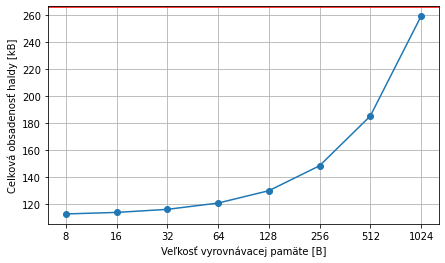
\includegraphics[width=\textwidth]{figures/verification/memory-usage-bytes.png}
     \end{subfigure}
     \hfill
     \begin{subfigure}[]{0.48\textwidth}
        \centering
     	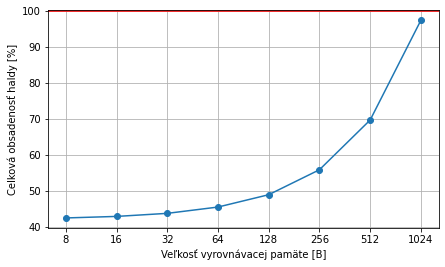
\includegraphics[width=\textwidth]{figures/verification/memory-usage-percentage.png}
     \end{subfigure}
     \caption{Celkové využitie dynamickej pamäte z haldy v DRAM}
\end{figure}

\begin{figure}[h]
	\centering
    \begin{subfigure}[]{0.48\textwidth}
    	\centering
        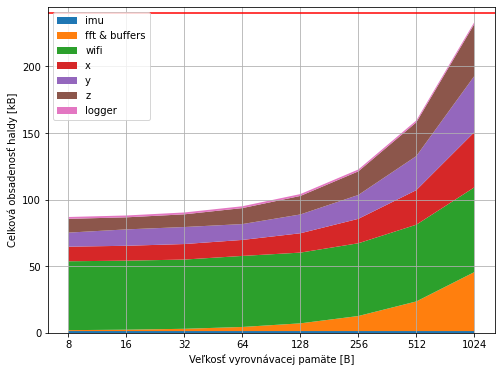
\includegraphics[width=\textwidth]{figures/verification/memory-profile-bytes.png}
        \caption{Celkový pamäťový profil}
     \end{subfigure}
     \hfill
     \begin{subfigure}[]{0.48\textwidth}
        \centering
     	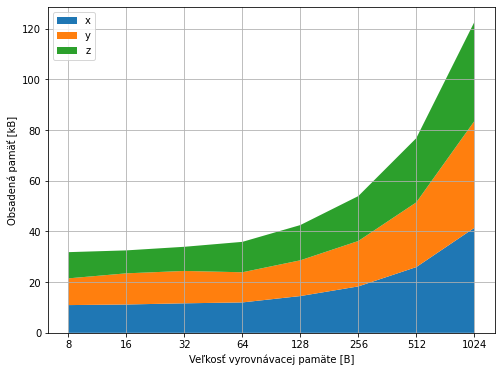
\includegraphics[width=\textwidth]{figures/verification/memory-profile-tasks.png}
     	\caption{Pamäťový profil úloh spracovania}
     \end{subfigure}
     \caption{Profil dynamickej pamäte}
\end{figure}

\url{https://blog.espressif.com/esp32-programmers-memory-model-259444d89387}

\section{Veľkosti prenášaných správ cez sieťové spojenie}
% tab. Réžia na MQTT

Maximálny počet udalostí, aby to bolo efektívne: Parametrická rovnica s parametrom počtom frekvenčných vedierok $n$ 
a počtom udalostí $p$ : $26 + 27 \cdot p < 5 \cdot n$. Percentuálny podiel udalostí: $p / n$. Pre $n = 16$: v priemere 
2 udalosti za okno ($12.5\%$). Pre $n = 512$: v priemere 93 udalostí za okno ($18.16\%$). Výhoda je predspracovanie, 
v tomto prípade aj dosiahneme menší počet prenesených dát. Štatistiky sa oplatí vytvárať pri najmenšom N = 32.

\begin{table}[h]
\def\arraystretch{1.25}
\begin{tabular}{|l|r|r|rr|cr|r|l}
\cline{1-8}
\multirow{2}{*}{\textbf{MQTT topic}} & \multicolumn{1}{c|}{\multirow{2}{*}{\textbf{\begin{tabular}[c]{@{}c@{}}Min. \\topic \end{tabular}}}} & \multicolumn{1}{c|}{\multirow{2}{*}{\textbf{\begin{tabular}[c]{@{}c@{}}Veľkosť\\ v RAM\end{tabular}}}} & \multicolumn{2}{l|}{\textbf{Hlavička (h)}}                      & \multicolumn{2}{l|}{\textbf{Prvok (p)}}                         & \multicolumn{1}{c|}{\multirow{2}{*}{\textbf{\begin{tabular}[c]{@{}c@{}}Max. celková\\ veľkosť\end{tabular}}}} & \textbf{} \\ \cline{4-7}
                                     & \multicolumn{1}{c|}{}                                                                                     & \multicolumn{1}{c|}{}                                                                                  & \multicolumn{1}{c|}{\textbf{Min.}} & \multicolumn{1}{c|}{\textbf{Max.}} & \multicolumn{1}{c|}{\textbf{Min.}} & \multicolumn{1}{c|}{\textbf{Max.}} & \multicolumn{1}{c|}{}                                                                                         &           \\ \cline{1-8}
config/response                      & 21                                                                                                        & 124                                                                                                    & \multicolumn{2}{c|}{-}                                                  & \multicolumn{1}{r|}{-}             & \multicolumn{1}{l|}{}              & 450                                                                                                           &           \\ \cline{1-8}
samples                              & 13                                                                                                        & 4n                                                                                                    & \multicolumn{1}{r|}{1}             & 3                                  & \multicolumn{2}{c|}{5}                                                  & h + e n                                                                                                      &           \\ \cline{1-8}
spectrum/+                           & 16                                                                                                        & 4(n/2)                                                                                                & \multicolumn{1}{r|}{14}            & 22                                 & \multicolumn{2}{c|}{5}                                                  & h + e(n / 2)                                                                                                 &           \\ \cline{1-8}
stats/+                              & 13                                                                                                        & 52                                                                                                     & \multicolumn{1}{r|}{4}             & 8                                  & \multicolumn{1}{r|}{9}             & 12                                 & 127                                                                                                           &           \\ \cline{1-8}
events/+                             & 14                                                                                                        & 20(n/2)                                                                                               & \multicolumn{1}{r|}{18}            & 26                                 & \multicolumn{1}{r|}{17}            & 27                                 & h + e(n / 2)                                                                                                &           \\ \cline{1-8}
\end{tabular}
\caption{Veľkosti správ pre MQTT topics}
\end{table}



\section{Čas vykonávania algoritmov}

\begin{table}[h]
\def\arraystretch{1.25}
\begin{tabular}{|l|l|l|l|l|l|l|}
\hline
\textbf{Veľkosť buffera}         & \textbf{32} & \textbf{64} & \textbf{128} & \textbf{256} & \textbf{512} & \textbf{1024} \\ \hline
\textbf{Štatistiky bez korelácii}& 3673        & 7471        & 14652        & 29574        & 59158        & 112871        \\ \hline
\textbf{DFT}                     & 80          & 162         & 306          & 611          & 1243         & 2620          \\ \hline
\textbf{DCT}                     & 91          & 165         & 310          & 612          & 1226         & 2532          \\ \hline
\textbf{Špičky: susedia}         & 45          & 102         & 216          & 451          & 913          & 1812          \\ \hline
\textbf{Špičky: nulou do záporu} & 6           & 10          & 17           & 33           & 62           & 121           \\ \hline
\textbf{Špičky: horský turista}  & 19          & 32          & 54           & 109          & 199          & 431           \\ \hline
\textbf{Udalosti}                & 7           & 10          & 17           & 31           & 58           & 114           \\ \hline
\end{tabular}
\caption{Čas vykonávania algoritmov od veľkosti vyrovnávacej pamäte v mikrosekundách pri taktovacej frekvencii 80 MHz a preemtívnom
ticku 100 Hz}
\end{table}

\begin{table}[h]
\def\arraystretch{1.25}
\centering
\begin{tabular}{|l|r|r|r|}
\hline
\textbf{N}  & \textbf{4} & \textbf{16} & \textbf{64} \\ \hline
\textbf{1x} & 108        & 262         & 891         \\ \hline
\textbf{4x} & 413        & 1041        & 3697        \\ \hline
\textbf{8x} & 819        & 2065        & 7209        \\ \hline
\end{tabular}
\caption{Čas v mikrosekundách na vyhladzovanie frekvenčného spektra v závislosti od veľkosti konvolučného jadra pri N = 512 a počtu opakovaných prechodov}
\end{table}


\section{Čas vykonávania pipeline}
Hraničný čas na dokončenie úlohy v reálnom čase v sekundách pre jednu vyrovnávaciu pamäť je $t \leq n / f_s$.
Podľa parametrickej nerovnice vieme určiť pre akú vzorkovaciu frekvenciu pri danej veľkosti okna je prekročená stanovená hranica:
$ f_s < n / t $. Všetky spracovania prebehnú do limitu zatiaľ čo sa zbiera druhé okno vzoriek. 

Hraničná najvyššia vzorkovacia pre double-buffer je pre jednu os spracovania 61,776 kHz a 12,785 kHz pre 3 osi spracovania.
Pre posielanie štatistík a spektra je max. vzorkovacia frekevencia 2,1 KHz, ale pri vyšších bufferoch sa pohybuje nad 7 KHz.
Pri 3 osiach spracovania je to max. 1320 Hz (N=32), 2510 Hz (N=256), 3741 Hz (N=1024)

\begin{table}[h]
\def\arraystretch{1.25}
\begin{tabular}{|l|l|r|r|r|}
\hline
\textbf{1 os}                 & \textbf{N}  & \textbf{32} & \textbf{256} & \textbf{1024} \\ \hline
\multirow{3}{*}{\textbf{DFT}} & \textbf{A1} & 518         & 2616         & 6401          \\ \cline{2-5} 
                              & \textbf{A2} & 435         & 1598         & 6209          \\ \cline{2-5} 
                              & \textbf{A3} & 467         & 1695         & 3864          \\ \hline
\multirow{3}{*}{\textbf{DCT}} & \textbf{A1} & 503         & 2117         & 4980          \\ \cline{2-5} 
                              & \textbf{A2} & 424         & 1012         & 3136          \\ \cline{2-5} 
                              & \textbf{A3} & 446         & 1064         & 3518          \\ \hline
\end{tabular}
\hfill
\begin{tabular}{|l|l|r|r|r|}
\hline
\textbf{3 osi}                 & \textbf{N}  & \textbf{32} & \textbf{256} & \textbf{1024} \\ \hline
\multirow{3}{*}{\textbf{DFT}} & \textbf{A1} & 2503        & 3077         & 10177         \\ \cline{2-5} 
                              & \textbf{A2} & 556         & 3340         & 10334         \\ \cline{2-5} 
                              & \textbf{A3} & 591         & 1295         & 4670          \\ \hline
\multirow{3}{*}{\textbf{DCT}} & \textbf{A1} & 667         & 1978         & 8485          \\ \cline{2-5} 
                              & \textbf{A2} & 518         & 1049         & 3720          \\ \cline{2-5} 
                              & \textbf{A3} & 572         & 1048         & 3897          \\ \hline
\end{tabular}
\caption{Čas na spracovanie okna vzoriek v mikrosekundách. Zariadenie v pokoji bez spracovania štatistík}
\end{table}


\begin{table}[h]
\def\arraystretch{1.25}
\begin{tabular}{|l|l|r|r|r|}
\hline
\textbf{}                       & \textbf{N}  & \textbf{32} & \textbf{256} & \textbf{1024} \\ \hline
\multirow{3}{*}{\textbf{1 os}}  & \textbf{A1} & 14750       & 34883        & 129190        \\ \cline{2-5} 
                                & \textbf{A2} & 8824        & 34351        & 139451        \\ \cline{2-5} 
                                & \textbf{A3} & 13795       & 34890        & 137346        \\ \hline
\multirow{3}{*}{\textbf{3 osi}} & \textbf{A1} & 23851       & 101978       & 273696        \\ \cline{2-5} 
                                & \textbf{A2} & 22981       & 78972        & 272161        \\ \cline{2-5} 
                                & \textbf{A3} & 24232       & 100156       & 270110        \\ \hline
\end{tabular}
\caption{Priemer z maxima z časov potrebných na spracovanie okna ktorejkoľvek osi spracovania. Posielanie štatistík s koreláciou a
frekvenčného spektra s FFT. RSSI je približne -40}
\end{table}


\section{Úspešnosť algoritmov na detekciu špičiek}
% Pri syntetických signáloch
% Tri pevné rovnomerne rozsotúpené frekvencie

% Náhodné frekvencie a trvania

% Accuracy algoritmu v tab. fs v N

% Best parametre algoritmu z grid search

\section{Spektrá a eventy v syntetických dátach}


\section{Obrázky spektier z reálnych datasetov}

\emptypage
